\documentclass[12pt]{article}
\usepackage[utf8]{inputenc}
\usepackage{graphicx}
\usepackage{amsmath}
\usepackage{hyperref}
\usepackage{amsfonts}
\usepackage{amssymb}
\usepackage{graphicx}
\usepackage{subcaption}
\usepackage{float}
\usepackage{tikz}
\usepackage{listings}
\usepackage{color}
\usepackage{parskip}
\usepackage{hyperref}
\hypersetup{
    colorlinks=true,
    linkcolor=black,
    citecolor=black,
    filecolor=black,
    urlcolor=black
}
\usepackage[left=1in,right=1in,top=1in,bottom=1in]{geometry}

\title{Rotacrypt: Rotational Mechanics as a Cryptographic Primitive}
\author{Teo Honda Scully}
\date{}

\begin{document}

\maketitle

\begin{abstract}
...TBD...
\end{abstract}

\tableofcontents

\newpage

\section{Introduction}

Ah, the Rubik's Cube—the iconic toy that bedevils and delights in equal measure. Born from the ingenious mind of Ernő Rubik in 1974, it's more than just a puzzle. Forget mere child's play; this cube is chaos in the physical. Just kidding. To go from the state of chaos to order, one only needs to know a solving protocol of which many exist.

\subsection{Review of Rubik's Cubes}

Max Park, the current world record holder (11 June 2023) for the 2-handed solve, obliterated the cube in a mind-blowing 3.13 seconds. Lucky scramble? Hardly. Yiheng Wang, who holds the world record average-of-five, clocks in at a dizzying 4.48 second mean solve time throughout the five solves.\footnote{An average-of-five is determined by taking the average of the three "middle" solves in a session of five scramble. In other words, the worst and best solve time are dropped from the calculation for the average.} And no, I won't depress you by mentioning his tender age of nine years old. But let's not divert. The Rubik's Cube--a mathematical marvel and a plaintext waiting to be encrypted. \\
\begin{figure}[h]
    \centering
    \begin{minipage}[c]{0.2\textwidth}
        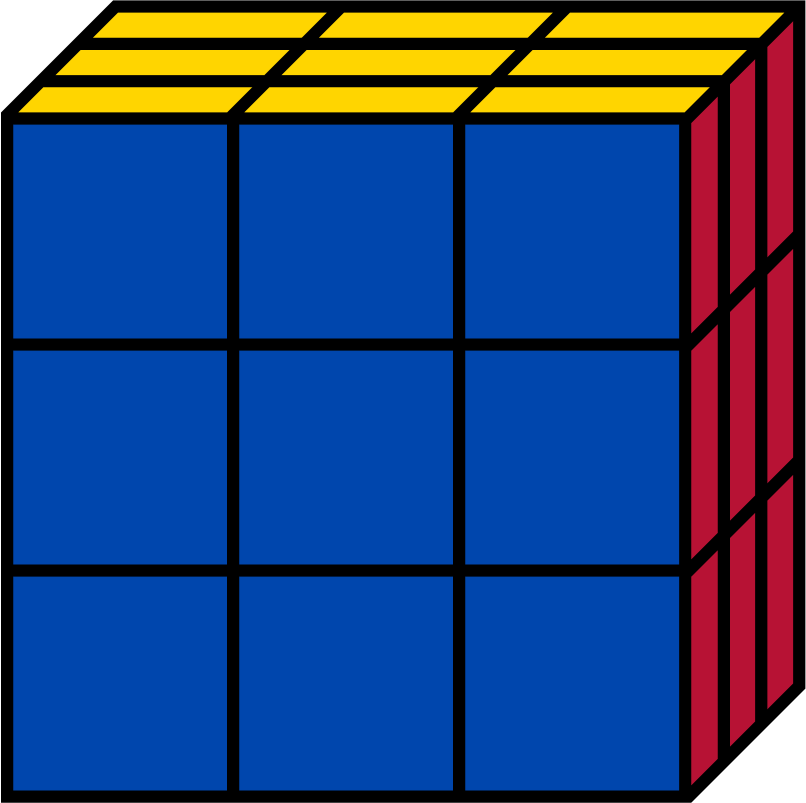
\includegraphics[scale=0.1]{cube.png}
    \end{minipage}
    \begin{minipage}[c]{0.2\textwidth}
        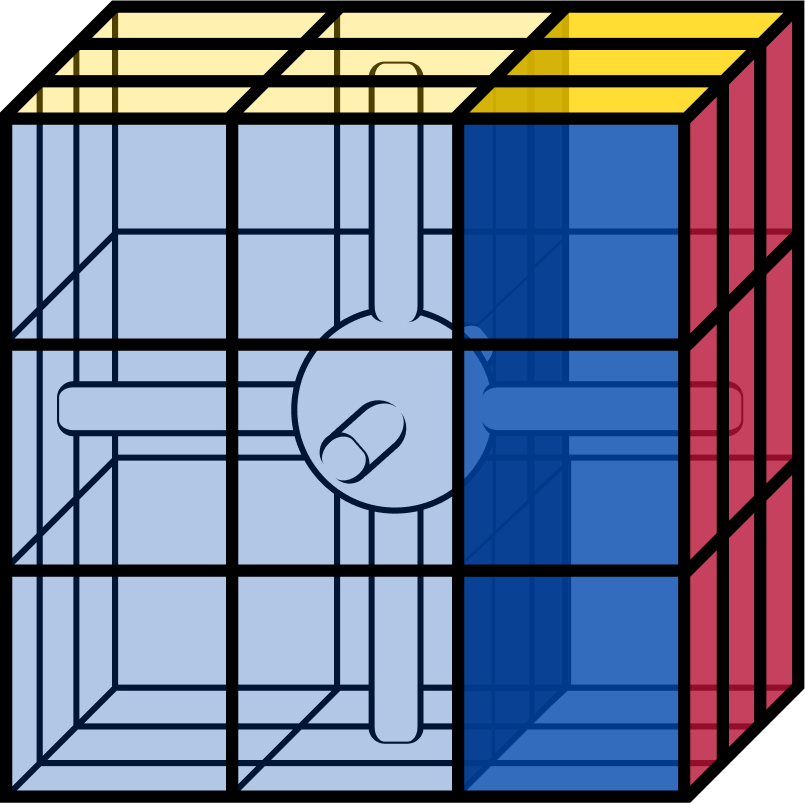
\includegraphics[scale=0.1]{moves/core_r_highlight.png}
    \end{minipage}
    \begin{minipage}[c]{0.05\textwidth}
        \centering
        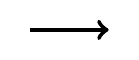
\begin{tikzpicture}
            \draw [->, ultra thick] (0,0.5)--(1,0.5);
        \end{tikzpicture}
    \end{minipage}
    \hspace{0.5cm}
    \begin{minipage}[c]{0.2\textwidth}
        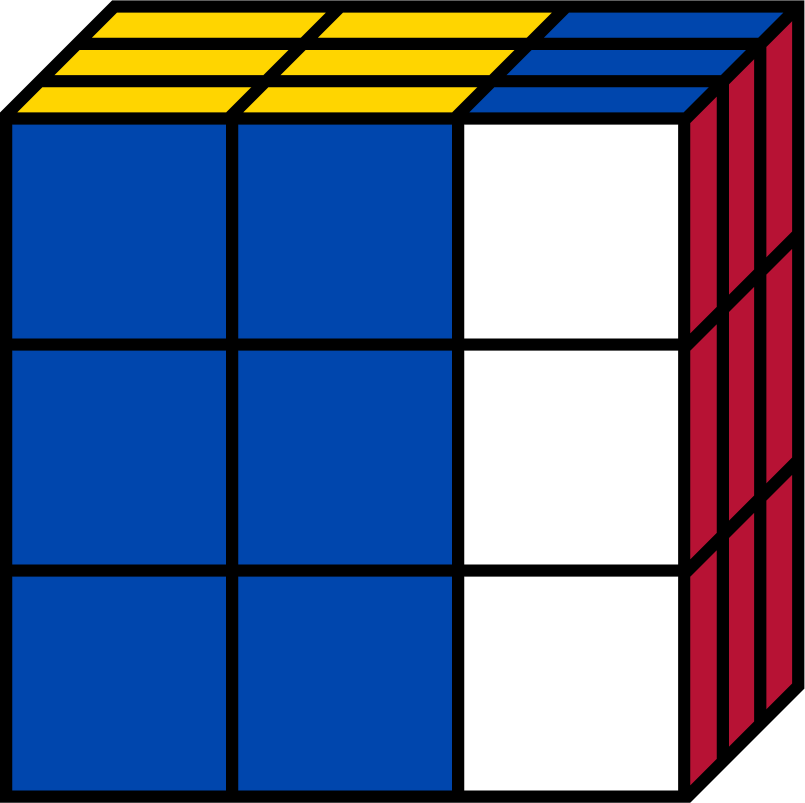
\includegraphics[scale=0.1]{moves/cube_r.png}
    \end{minipage}
    \begin{minipage}[c]{0.2\textwidth}
        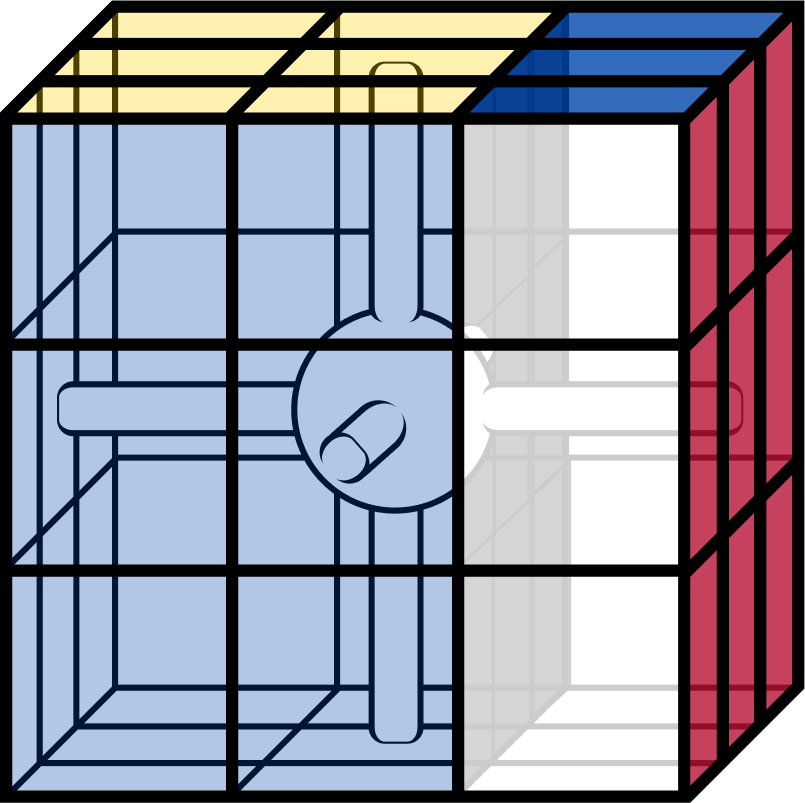
\includegraphics[scale=0.1]{moves/core_r_transform.png}
    \end{minipage}
    \caption{A visualization of the \textit{R} operation (rotating the right layer clockwise).}
\end{figure}

Let's dive into the mechanics of the 3x3x3 puzzle. The cube boasts centers, edges, and corners. These single-colored center pieces serve as the invariant axis around which the peripheral cubies rotate.\footnote{The smaller individual blocks that make up a Rubik's Cube are referred to as cubies.} The six unit colors are yellow, blue, red, green, orange, and white.

\begin{figure}[h]
    \hfill 
    \begin{minipage}[c]{0.2\textwidth} 
        \centering
        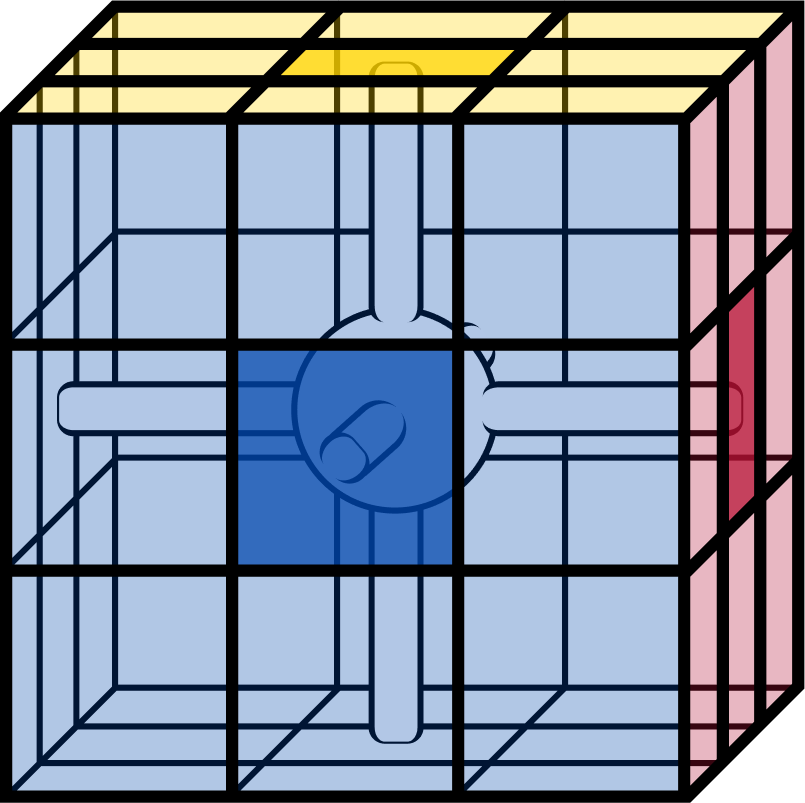
\includegraphics[scale=0.1]{moves/core.png}
    \end{minipage}
    \hfill 
    \begin{minipage}[c]{0.59\textwidth} 
        \vspace*{\fill} 
        A visualization of a 3x3x3 cube. The cube has 6 faces, each with 9 stickers. Notably, this means that there exists 54 different unit tiles on the cube. The cube has 43,252,003,274,489,856,000 possible states.\footnotemark
        \vspace*{\fill}
    \end{minipage}
    \hfill 
\end{figure}
\footnotetext{This number is calculated by considering the \( 8 \) corners, each with \( 3 \) orientations, and the \( 12 \) edges, each with \( 2 \) orientations.}

For instance, if the cube is held with a yellow top and blue front, the red and orange faces will invariably be to the right and left, respectively. In fact, the red and orange center pieces will \textit{always} be opposites, as will the blue-green and white-yellow pairs of center pieces.\\

\begin{figure}[h]
    \centering
    \begin{minipage}[c]{0.2\textwidth}
        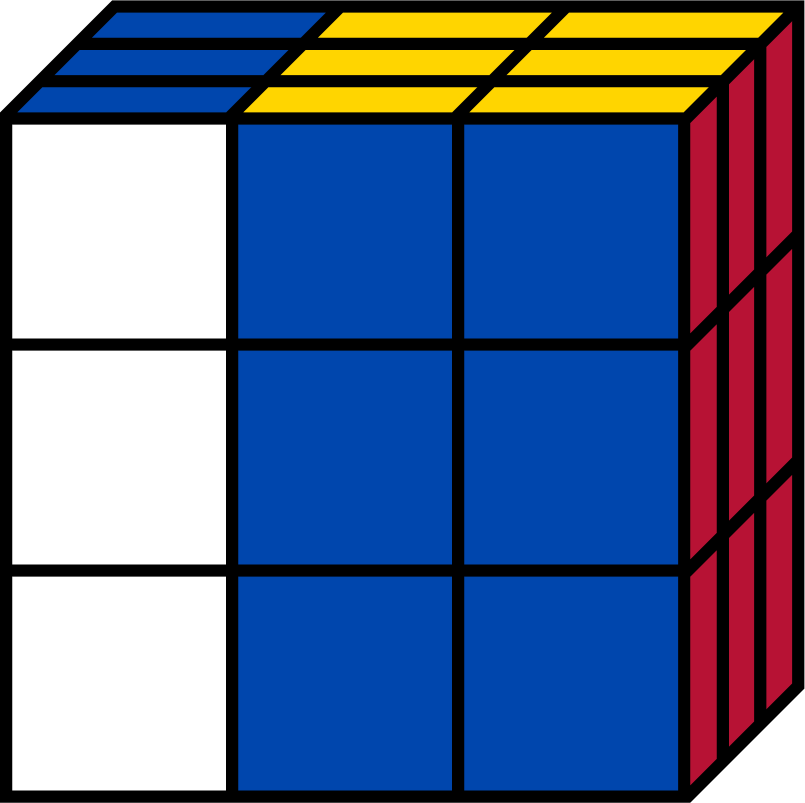
\includegraphics[scale=0.1]{moves/cubeLp.png}
    \end{minipage}
    \begin{minipage}[c]{0.05\textwidth}
        \centering
        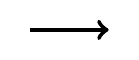
\begin{tikzpicture}
            \draw [->, ultra thick] (0,0.5)--(1,0.5);
        \end{tikzpicture}
    \end{minipage}
    \hspace{0.5cm}
    \begin{minipage}[c]{0.2\textwidth}
        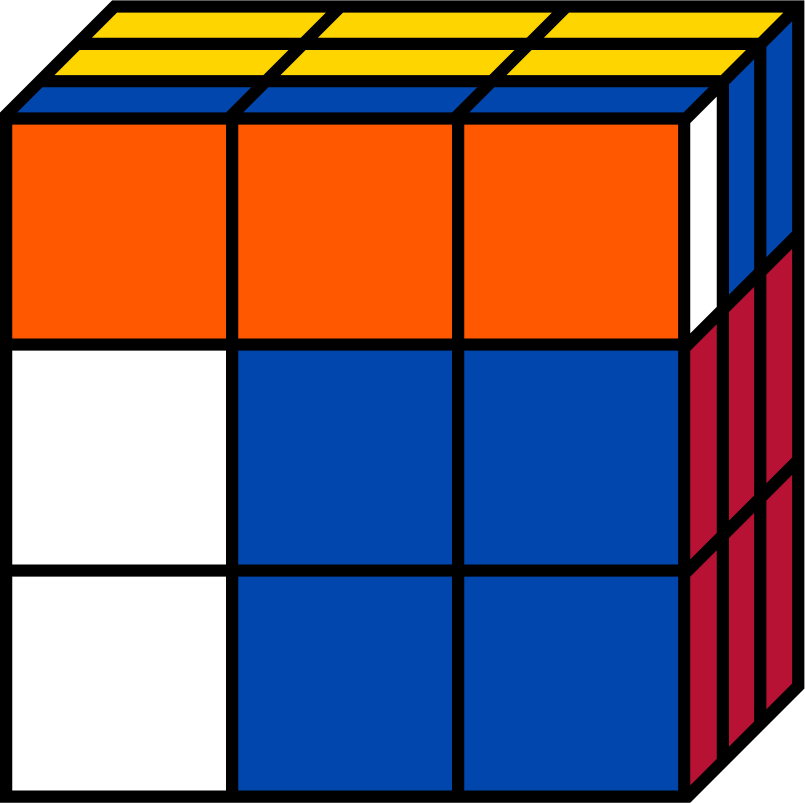
\includegraphics[scale=0.1]{moves/cubeLpUp.png}
    \end{minipage}
    \begin{minipage}[c]{0.05\textwidth}
        \centering
        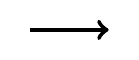
\begin{tikzpicture}
            \draw [->, ultra thick] (0,0.5)--(1,0.5);
        \end{tikzpicture}
    \end{minipage}
    \hspace{0.5cm}
    \begin{minipage}[c]{0.2\textwidth}
        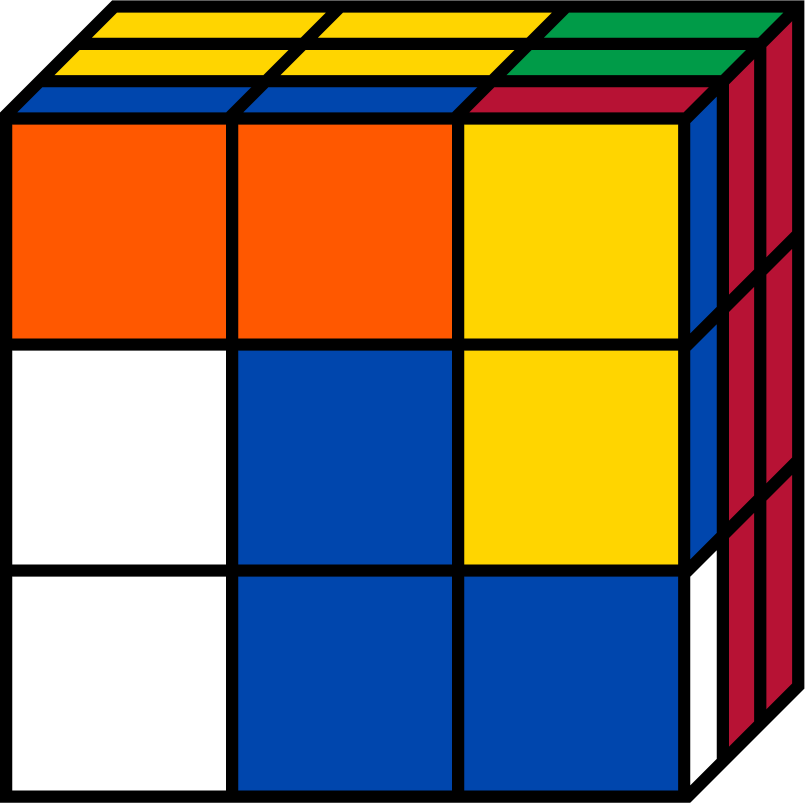
\includegraphics[scale=0.1]{moves/cubeLpUpRp.png}
    \end{minipage}
    \caption{A visualization of the \textit{L' U' R'} operation(s).}
\end{figure}

\subsection{Notation for Cube Operations}

The notation used to describe the movements and algorithms for solving the Rubik's Cube is standardized to facilitate easy understanding and sharing of solutions. Each face of the cube is designated by an uppercase letter:

\begin{itemize}
    \item \textbf{U} - Up (Top Layer)
    \item \textbf{D} - Down (Bottom Layer)
    \item \textbf{L} - Left (Left Layer)
    \item \textbf{R} - Right (Right Layer)
    \item \textbf{F} - Front (Front Layer)
    \item \textbf{B} - Back (Back Layer)
\end{itemize}

The following symbols are appended to these letters to indicate the direction of rotation:

\begin{itemize}
    \item No symbol - 90-degree clockwise rotation
    \item \textbf{'} (apostrophe) - 90-degree counterclockwise rotation
    \item \textbf{2} - 180-degree rotation (either direction)
\end{itemize}

For example, the sequence \textit{L' U' R'} would indicate a counterclockwise rotation of the left layer, followed by a counterclockwise rotation of the top layer, and finally, a counterclockwise rotation of the right layer.

\subsection{God's Number}
In the realm of 3x3x3 Rubik's Cubes, \textit{God's Number} is a term used to denote the maximum number of moves required to solve any scrambled cube. It has been proven that any cube can be solved in 20 moves or fewer (the citation can be found in the \textit{References} section). This concept is an intriguing insight into the mathematical efficiency of the cube's design.

Furthermore, this means that any scramble can be reached with 20 moves or fewer. This is a key point to keep in mind when considering the security of the cube as a cryptographic primitive as well as for key size considerations.\\

\subsection{Combinatorial Explosion with Multiple Cubes}
Let us consider the number of possible states for a single 3x3x3 Rubik's Cube, which is \(43,252,003,274,489,856,000\). When chaining together the combinations of two different cubes, the number of combined states is \((43,252,003,274,489,856,000)^2\).

This squaring occurs because each state of the first cube can pair with every state of the second cube, yielding \(43,252,003,274,489,856,000 \times 43,252,003,274,489,856,000\). Mathematically, the set of possible states becomes the Cartesian product of the two sets of states, leading to an exponential increase in complexity.

One intriguing aspect of chaining multiple Rubik's Cubes is the exponential growth in the state space. Let \( N \) represent the number of unique states for a single Rubik's Cube. For \( k \) chained Rubik's Cubes, the total number of unique states becomes \( N^k \). This exponential increase serves a critical function: it substantially minimizes the likelihood of collisions whilst simultaneously increasing the difficulty of brute-force attacks.

\subsection{Edge and Corner Constraints}

While the utilization of multiple Rubik's Cubes in the encryption scheme introduces a combinatorial explosion in the state space, it is essential to consider the limitations imposed by the unique mapping of plaintext bits to cube pieces. In this scheme, each plaintext bit (either a 0 or 1) is mapped to a specific piece on the cube, which can either be an edge or a corner.

One of the fundamental constraints of a Rubik's Cube is that edges and corners are immutable in their categories; edges cannot morph into corners and vice versa. Due to this constraint, it becomes inappropriate to assign all 48 movable units (54 total units minus 6 centers) to represent bits, as doing so would leave patterns in trivial plaintext-to-ciphertext cryptanalysis attacks. If a bit mapped to a corner unit can never be encrypted into an edge piece no matter how many layer operations occur, this serves as a trivial pattern in which cryptanalysists can exploit.

\subsection{Per-Cube 24-bit State Space}
As a result of the aforementioned limitations, the encryption scheme opts for a more constrained assignment by sticking to either edges or corners to represent the bits. This decision narrows down the number of units used for bit representation to 24, thus limiting the state space to \(2^{24}\) for each cube.

Given the inherent limitations in the state space of a single Rubik's Cube, capped at \(2^{24}\) due to geometric constraints, a novel approach to enlarging this space involves chaining multiple cubes together. Specifically, by employing a tuple of six Rubik's Cubes for each block, the scheme effectively increases the state space to \(2^{(24 \times 6)}\).

In this enhanced scheme, each block of plaintext is split into six portions, each of which is mapped onto a separate cube. The combined state of all six cubes serves as a unique representation of the original block. This approach leverages the geometric diversity across multiple cubes to create a more complicated and less predictable state space.

The chaining of six cubes per block substantially complicates the task of deciphering the ciphertext without knowledge of the encryption key, thereby augmenting the cryptographic strength of the scheme. With a state space of \(2^{(24 \times 6)}\), the algorithm becomes computationally prohibitive for brute-force attacks, even when accounting for potential parallelization.

While the increase in state space significantly boosts the algorithm's resilience against attacks, it also introduces additional computational complexity. However, the impact on efficiency is deemed acceptable given the substantial increase in cryptographic security.

\subsection{Summary}

The \textit{Introduction} can be summarized with the following points:

\begin{itemize}
    \item \textbf{3x3x3 Mechanics}: The cube boasts centers, edges, and corners. The six unique single-colored center pieces serve as the invariant axis around which the peripheral cubies rotate.
    \item \textbf{State Space}: The cube has 6 faces, each with 9 stickers. Notably, this means that there exists 54 different unit tiles on the cube. The cube has 43,252,003,274,489,856,000 possible states.
    \item \textbf{Increasing State Space}: Let \( N \) represent the number of unique states for a single Rubik's Cube. For \( k \) chained Rubik's Cubes, the total number of unique states is \( N^k \). 
    \item \textbf{No More Colors}: In this scheme, colors are not mapped to units on the cube. Instead, each plaintext bit (either a 0 or 1) is mapped to a specific piece on the cube. As centers are immutable, they are not used to represent bits (only 48 movable units).
    \item \textbf{Mapping Constraints}: One should note that edges cannot morph into corners and vice versa. Therefore, bits are only assigned exclusively to either edges or corners (24 potential bit mappings per cube), thus limiting the state space to \(2^{24}\) for each cube.
    \item \textbf{Increasing State Space Again}: By employing a tuple of six Rubik's Cubes for each block, the scheme effectively increases the state space to \(2^{(24 \times 6)}\), yielding \(2^{144}\) possible states per cube.
\end{itemize}

\newpage

\section{Overview}

The proposed encryption scheme is a block cipher that leverages the mathematical complexities and state space of Rubik's Cubes. Each block in the scheme utilizes a tuple of six 3x3x3 Rubik's Cubes, effectively rendering a block size of 144 bits (24 bits per cube; 6 cubes).

\subsection{Initial Round}

At the start of the encryption process, each cube is initialized to the solved state and then a corresponding-plaintext-bit-to-3x3x3-layer-operation-mapping is applied. The details of this progress can be found in the \textit{Encryption / Cube Mapping Procedure} section. This will yield six unique cube states.

\begin{figure}[H]
    \centering
    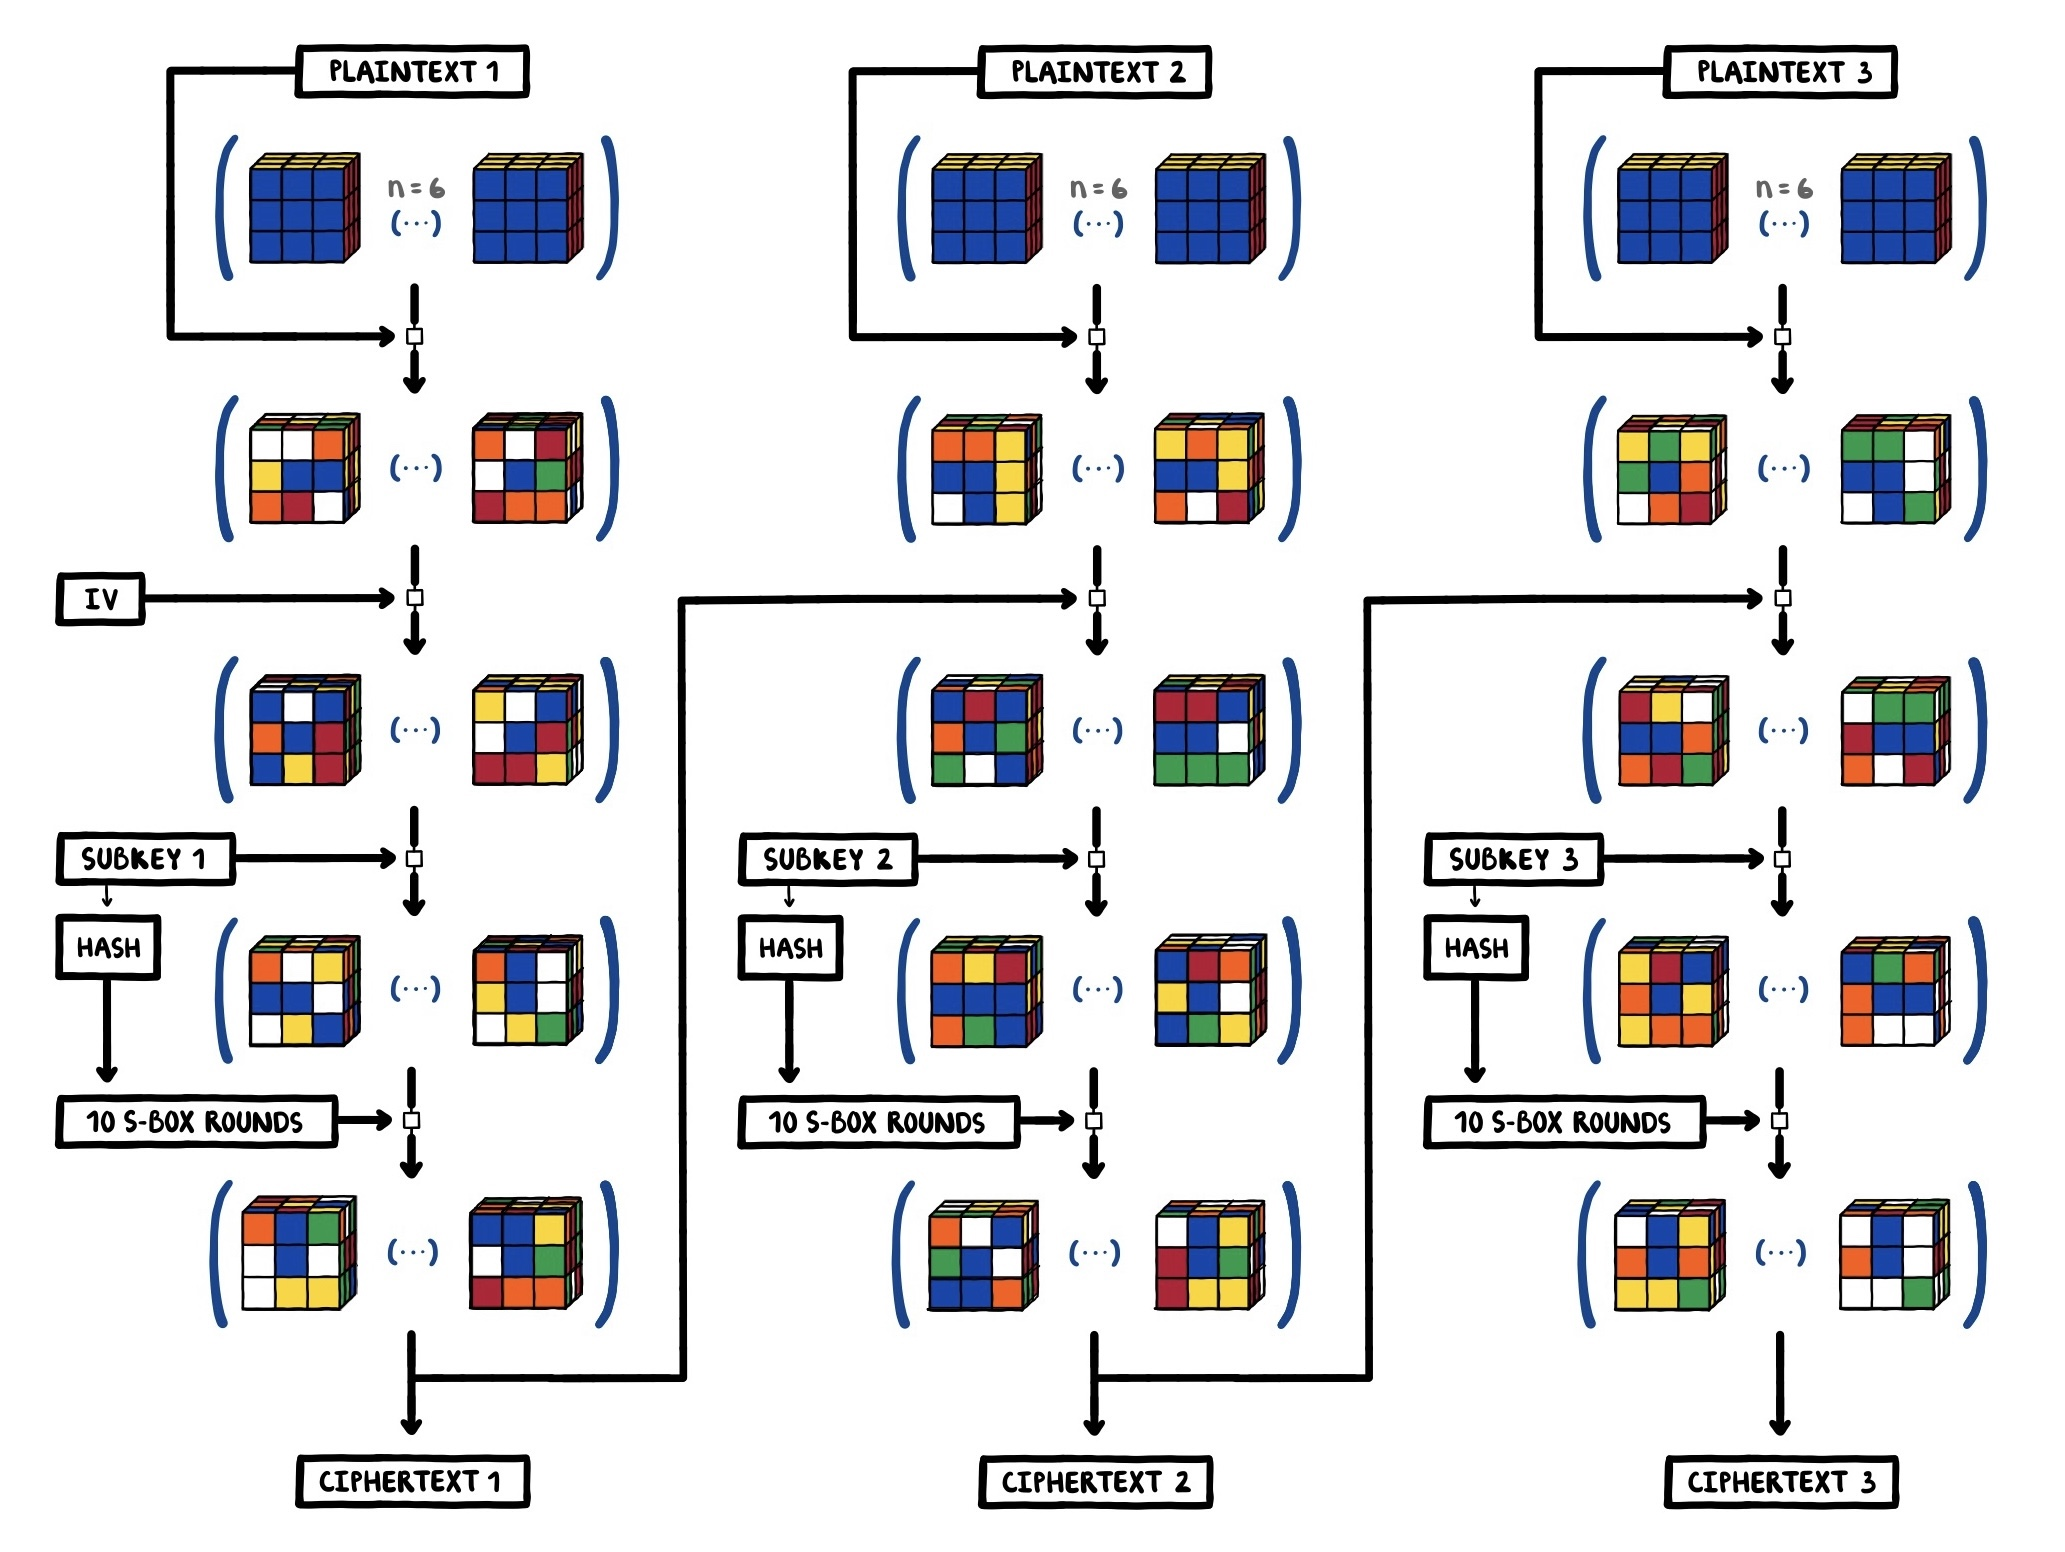
\includegraphics[width=\textwidth]{encryption/encryption.jpg}
    \caption{Rotacrypt Encryption Overview}
\end{figure}

The initial round begins by applying a cryptographically secure pseudorandom number generated Initialization Vector (IV) deserialized into six unique scrambles. Each cube in the tuple will have their own unique scramble at this stage, and a dynamic subkey is then generated from the original key using a secure key derivation function. The subkey is likewise deserialized into six unique scrambles. Each scramble is applied to their respective cube. The cubes finally undergo a series of deterministic Rubik's moves, mimicking the traditional S-box and diffusion operations in AES like SubBytes, ShiftRows, and MixColumns. These Rubik's moves are termed as SubCubes, ShiftFaces, and MixEdges respectively. It should be noted that the nature of layer operations intrinsically involves a form of diffusion, making the scheme's diffusion already naturally high without S-box operations. The resultant state of the cubes serves as the ciphertext for that block.

One may question the intent of an S-box operation if the layer operations already provide a high degree of diffusion. Layer operations are linear transformations (this becomes evident in \textit{3x3x3 Implementation}), and the S-box operation adds a layer of non-linearity to the encryption process. This non-linearity is critical to the security of the scheme, as it prevents the encryption process from being modeled as a linear system of equations. 

\vspace{0.5cm}

\textbf{\textit{Relevant Definitions}}:

\begin{itemize}
    \item \textbf{S-box}: A substition box is a cryptographic component that performs fixed, non-linear substitutions on input bits to produce output bits.
    \item \textbf{Plaintext and Ciphertext}: In cryptography, plaintext refers to the original readable message, while ciphertext is the scrambled message produced through encryption.
    \item \textbf{State Space}: The state space refers to the total number of possible configurations or states that a system can be in; for a cube, it's a very large number. Maybe not yet large enough?
    \item \textbf{Six Cube Tuple}: In this scheme, a tuple refers to an ordered set of six individual Rubik's Cubes, each contributing to the encryption process.
    \item \textbf{Brute-force attacks}: In cryptography, a brute-force attack involves trying all possible combinations to decrypt a message, which is computationally expensive.
    \item \textbf{Parallelization}: Parallelization refers to the process of dividing a task into sub-tasks that are solved concurrently, often used to speed up computational tasks.
    \item \textbf{Cryptographic Security}: The term refers to the resilience of a cryptographic system against unauthorized access or data breaches.
    \item \textbf{Mapping Constraints}: In this scheme, mapping constraints refer to the limitations in how data can be represented on the cube, such as not being able to interchange edges and corners.
    \item \textbf{Geometric Constraints}: These are the limitations imposed by the physical structure of the Rubik's Cube, like the inability to change an edge piece into a corner piece.
    \item \textbf{Cryptanalysis Attacks}: Cryptanalysis attacks involve mathematical and computational techniques to analyze and possibly break an encryption scheme.
\end{itemize}

\subsection{Subsequent Rounds}
For subsequent rounds, a part of the cube state from the previous round is extracted and used as the IV for the next block. New subkeys are generated dynamically by hashing the original key along with a salt (detailed in the \textit{Key Generation / Sub-Key Generation} section), which is then converted into a Rubik's Cube scramble sequence. The same sequence of operations: SubCubes, ShiftFaces, and MixEdges, are then applied to these new blocks, followed by scrambling with the round-specific subkey.

The state of the cubes after the S-box operation is used to link subsequent blocks, ensuring that the entire encryption process influences each block. This design decision not only maximizes the use of the large Rubik's Cube state space but also provides strong cryptographic properties.

We are chaining blocks to increase diffusion. A blockchain if you must.
\subsection{Final Round}

(MAYBE... TBD) In the final round, the processed cubes go through an S-box transformation to further improve the security of the encrypted data. This S-box is carefully designed to maximize non-linearity and is dynamically generated based on the cube's final state.

\subsection{Purpose}
There is no purpose. I was told not to make a cryptosystem, so I did the opposite.

\subsection{Intended Usage}
<...>

\section{3x3x3 Implementation}
<...>

\subsection{Data Structure Breakdown}
<...>

\subsection{Augmented SPEFFZ Mapping}
<...>

\subsection{Cyclic Transformations}

\section{Key Generation}

\begin{figure}[H]
    \centering
    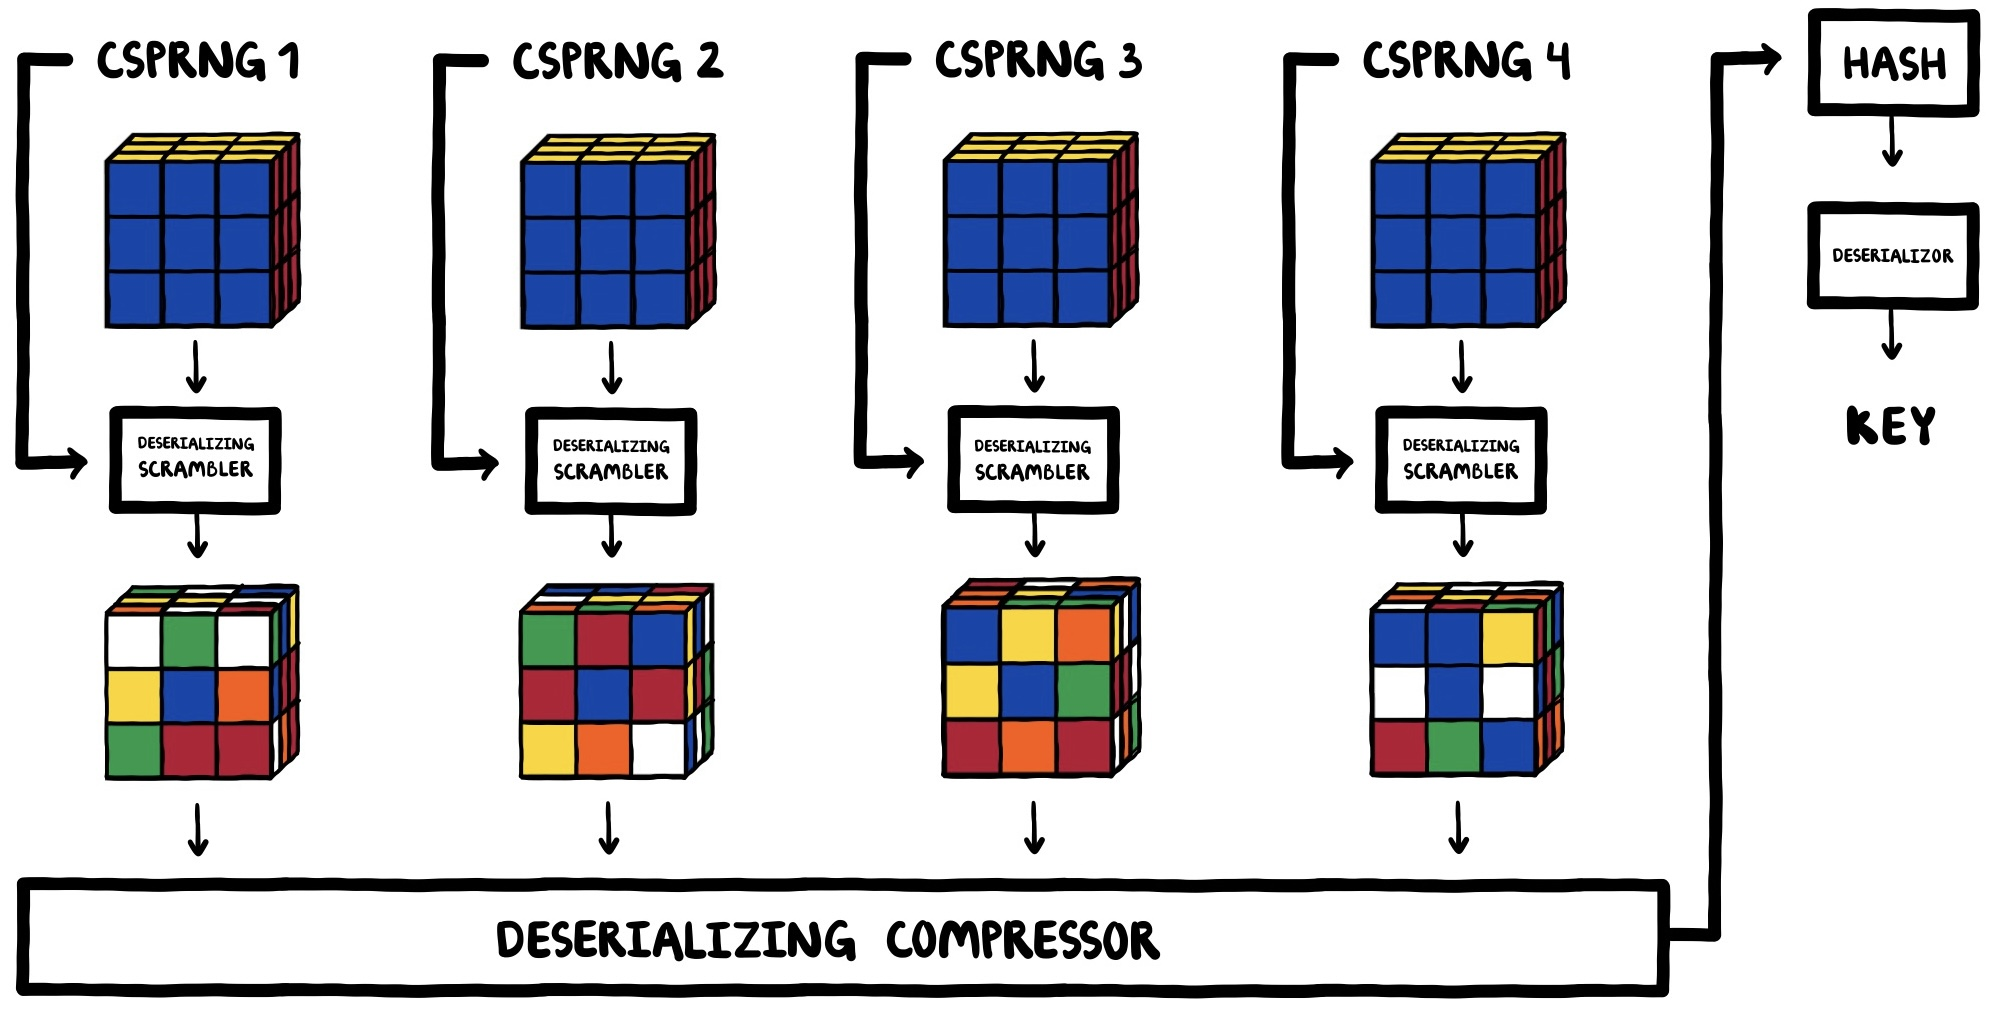
\includegraphics[width=\textwidth]{key_gen/keygen.jpg}
    \caption{beep boop}
\end{figure}

\subsection{4-Cube Initialization}
<...>

\subsection{Master-Key Serialization}
<...>

\subsection{Sub-Key Generation}
<...>

\section{Encryption}
<...>

\subsection{Plaintext Setup With S-Box Transformations On Chunks}
<...>

\subsection{Cube Mapping Procedure}
<...>

\subsection{Encryption Algorithm}
<...>

\section{Decryption}

\subsection{Beep Boop}

\section{Security Analysis}

\subsection{Immediate Reduction to AES}

\section{Codebase Architecture}

\subsection{Architecture Tree}

\end{document}
